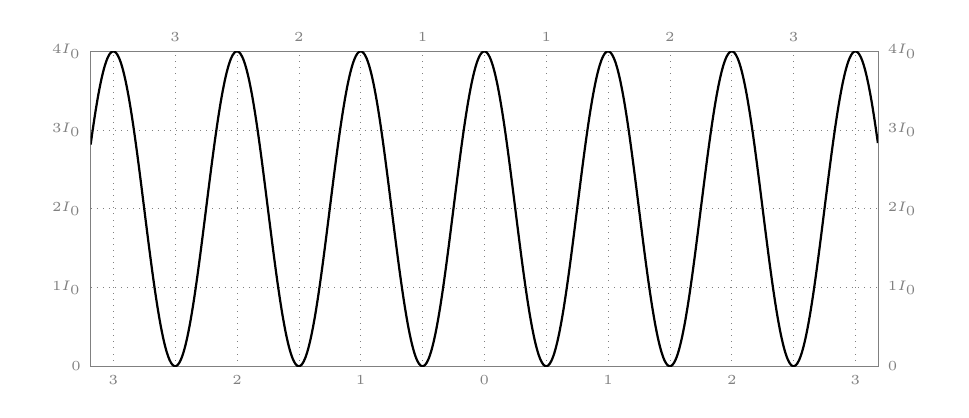
\begin{tikzpicture}

\tikzset{aux/.style={gray,very thin,dotted}}

\clip(-5.8,-0.3) rectangle (5.8,4.3);

\draw[gray] (-5,0) rectangle (5,4);

\foreach \x in {-3,-2.5,...,3}
{
    \draw[aux](\x*pi/2,0)--(\x*pi/2,4);
}

\foreach \x in {1,2,3}
{
    \draw[aux] (-5,\x)--(5,\x);
}

\begin{scope}
    \clip (-5,0) rectangle (5,4);
    \draw[thick] plot[domain=-5:5,smooth,samples=500] (\x,{2*cos(deg(4*\x))+2});
\end{scope}

\path (-5,0) node[left,gray] {\tiny $0$};
\path (-5,1) node[left,gray] {\tiny $1I_0$};
\path (-5,2) node[left,gray] {\tiny $2I_0$};
\path (-5,3) node[left,gray] {\tiny $3I_0$};
\path (-5,4) node[left,gray] {\tiny $4I_0$};

\path (5,0) node[right,gray] {\tiny $0$};
\path (5,1) node[right,gray] {\tiny $1I_0$};
\path (5,2) node[right,gray] {\tiny $2I_0$};
\path (5,3) node[right,gray] {\tiny $3I_0$};
\path (5,4) node[right,gray] {\tiny $4I_0$};

\foreach \x in {-3,-2,...,3}
{
    \path(\x*pi/2,0) node[below,gray] {\tiny $\fpeval{abs(\x)}$};
}

\foreach \x in {1,2,3}
{
    \path(+\x*pi/2-pi/4,4) node[above,gray] {\tiny $\fpeval{\x}$};
    \path(-\x*pi/2+pi/4,4) node[above,gray] {\tiny $\fpeval{\x}$};
}

\end{tikzpicture}
